\section{Lexical Functional Grammar (LFG)}

\subtitle{Lexical Functional Grammar (LFG)}

\huberlintitlepage[22pt]


\outline{

\begin{itemize}
\item Introduction and basic terms
\item Phrase structure grammar and \xbar Theory
\item Government \& Binding (GB)
\item {Generalized Phrase Structure Grammar (GPSG)}
\item {Feature descriptions, feature structures and models}
\item \alert{Lexical Functional Grammar (LFG)}
%\item PATR
\item Categorial Grammar (CG)
\item Head-Driven Phrase Structure Grammar (HPSG)
%\item Konstruktionsgrammatik (CxG)
\item Tree Adjoning Grammar (TAG)
\end{itemize}

%\tableofcontents
}

\frame{
\frametitle{Reading material}

\citew[Chapter~7]{MuellerGT-Eng} (without 7.1.5 on semantics)

}

\exewidth{(123)}


\frame{
\frametitle{Lexical Functional Grammar (LFG)}


\begin{itemize}[<+->]
\item Developed by Joan Bresnan and Ron Kaplan in the 1980s.\nocite{BK82a}

\item LFG is part of so-called West-Coast-Linguistics:\\
      Joan Bresnan (LFG) and Ivan Sag (HPSG) did their PhD with Chomsky\\
      (MIT is situated at the East Coast of the US,\\
       while Stanford, Palo Alto and Berkeley are in the Bay Area in California)

\item LFG aims for psycholinguistical plausibility and wants to be implementable

\item teaching material and overview articles:
      \citew{BATW2016a,Dalrymple2006a}

\item In-depth works on German: \citew{Berman96a-u,Berman2003a} and \citew{Cook2001a}

\end{itemize}

}


\subsection{General remarks on the representational format}

\frame{
\frametitle{General remarks on the representational format}

\begin{itemize}
\item multiple levels of representation:
      \begin{itemize}
      \item c-structure (constituent structures, licensed by PSG, \xbar structures)
\pause
      \item f-structure (functional structure)
      \end{itemize}
\pause
\item Mappings relate c- and f-structure.
\end{itemize}

}

\subsubsection{Functional structure}


\subsubsubsection{Grammatical functions}

\frame[shrink=10]{
\frametitle{Grammatical functions and f-structure}


In LFG, grammatical functions (subject, object, \ldots) play a very important role.\\
They are primitives of the theory.

\pause


A sentence such as (\mex{1}a) has the functional structure in (\mex{1}b):
\eal
\ex David devoured a sandwich.
\ex \lfgms{ pred & `devour\sliste{\lfgsubj,\lfgobj}'\\
         subj & \lfgms{ pred &  `David' \\
                   }\\
         obj  & \lfgms{ spec & A\\
                     pred & `sandwich'\\
                   }\\
       }
\zl

All lexical items that have a meaning (\eg nouns, verbs, adjectives) contribute a
\textsc{pred} feature with a corresponding value.

The grammatical functions governed by a head (government = subcategorization)
are determined in the specification of \textsc{pred}.

}

\frame{
\frametitle{Governable grammatical functions}

The respective grammatical functions are called \emph{governable grammatical functions}.

Examples:

\begin{tabular}[t]{@{}lp{26em}@{}} 
\sc subj: & subject \\ 
\pause
\sc obj: & object\\ 
\pause
%% \sc comp: & Satz- oder abgeschlossenes (nicht-prädikatives) Infinitivkomplement\\
\sc comp & sentential complement\\
%% \sc xcomp: & offenes (prädikatives) Komplement, oft infinitivisch, dessen {\sc subj}"=Funktion
%% extern kontrolliert wird\\
\objtheta: & secondary \textsc{obj} functions that are related to a special, language \\
           & specific set of grammatical roles; English has \objtheme only.\\
%
\obltheta: & a group of thematically restricted oblique functions, as for instance
         {\obl\downlett{GOAL}} or {\obl\downlett{AGENT}}. These often correspond to adpositional
         phrases in c-structure.\\
\end{tabular}

}

\frame{
\frametitle{Non-governable grammatical functions}

Apart from this there are non-governable grammatical functions.

Examples:
\begin{tabular}[t]{@{}lp{26em}@{}} 
\textsc{adj}: & adjuncts \\ 
%
\textsc{topic}: & the topic of an utterance\\ 
%
\textsc{focus}: & the focus of an utterance\\
\end{tabular}



}

\subsubsubsection{Functional descriptions}



\frame{
\frametitle{Functional descriptions}


Reference to a value of the feature \textsc{tense} in the functional structure $f$:
\ea
($f$ \lfgtense)
\z

\pause

It is possible to say something about the value which this feature should have in the feature description.
\ea
($f$ \lfgtense) = \lfgpast
\z

\pause

The value of a feature may also be a specific f"=structure. The expression in (\mex{1})
ensures that the \subjf in $f$ is the f"=structure $g$:

\ea
($f$ \lfgsubj) = $g$
\z

}

\frame[shrink]{
\frametitle{Descriptions and f-structures}
\eal
\ex David sneezed.
\ex 
\begin{tabular}[t]{l}
($f$ \lfgpred) = {\small `SNEEZE\sliste{\lfgsubj}'}\\
($f$ \lfgtense) = {\small PAST}\\
($f$ \lfgsubj) = $g$\\
($g$ \lfgpred) = {\small `David'}
\end{tabular}
\zl

\pause
The description in (\mex{0}b) describes the following structure:

\ea
$f$: \lfgms{ pred  & `SNEEZE\sliste{\lfgsubj}'\\
          tense & PAST\\
          subj  & $g$: \onems{ pred `David' }\\
        }
\z

(\mex{-1}b) also describes many other structures which contain further features.\\
We are only interested in minimal structures containing the information provided in the description.

}


\exewidth{(100)}
\frame{
\frametitle{Mappings from c-structure to f-structure}

\eal
\ex David sneezed.
\ex 
\tree{IP}{%
  \tree[b]{NP}{\tree{N$'$}{\tree{N}{\le{David}}}}
  \tree{I$'$}{\tree{VP}{\tree{V$'$}{\tree{V}{\le{sneezed}}}}}}%
\hspace*{4em}%
\raisebox{-2em}{\lfgms{
pred & `SNEEZE\sliste{\lfgsubj}'\\
tense & PAST\\
subj  & \rnode{i}{\lfgms{ pred & `David' \\
                      }}\\
}}\\
\ltor[-15]{b}[175]{i}
\Aput*{$\phi$}
\zl


A phrase and its head always correspond to the same f"=structure.\\
IP, I$'$ and I (and also VP) are mapped onto the same f"=structure.

}


\frame{
\frametitle{Heads and f-structure}

A phrase and its head always correspond to the same f"=structure:

\ea
\begin{tabular}[t]{@{}c@{}}
\rnode{a}{\rnode{v1}{V$'$}}\\[2ex]
\rnode{b}{\rnode{v}{V}}\\[2ex]
\rnode{sneezed}{sneezed}\\
\end{tabular}
\hspace*{4em}
\rnode{d}{\raisebox{-2em}{\fd{\fdand{\feat{\lfgpred}{\small `SNEEZE\sliste{\lfgsubj}'}
                    \feat{\lfgtense}{\small PAST}}}}}
\ncline{v1}{v}\ncline{v}{sneezed}%
\ltor{a}{d}
\Aput*{$\phi$}
\ltor{b}{d}
\z

}


\frame{
\frametitle{IP, I$'$, I and VP are mapped to the same f-structure}



In LFG grammars of English, the CP/IP system is assumed as in \gbt. IP, I$'$ and I
(and also VP) are mapped onto the same f"=structure.
\eal
\ex David is yawning.

\ex {\tree[a]{IP}{%
  \tree{NP}{\tree{N$'$}{%
    \tree{N}{\le{\em David}}}}
  \tree[b]{I$'$}{%
    \tree[c]{I}{\le{\em is}}
    \tree[d]{VP}{\tree[e]{V$'$}{\tree[f]{V}{\le{\em yawning}}}}}}}%
\hspace*{4em}%
{\rnode{o}{\raisebox{-2em}{\fd{\fdand{\feat{\lfgpred}{\small `YAWN\sliste{\lfgsubj}'}
                    \feat{\lfgtense}{\small PRES}
           \feat{\lfgsubj}{\fdand{\feat{\lfgpred}{\small `David'}}}}}}}}
\ltor{a}{o}
\ltor{b}{o}
\ltor[10]{c}{o}
\ltor{d}{o}
\ltor{e}{o}
\ltor{f}{o}
\zl

}



%% \subsubsection{Funktionale Eindeutigkeit ({\em Functional Uniqueness})}

%% \frame{
%% \frametitle{Funktionale Eindeutigkeit ({\em Functional Uniqueness})}

%% }

\subsubsection{Completeness}

\frame{
\frametitle{Completeness}

Elements required in the \textsc{pred} value have to be realized.

\eal
\ex[*]{David devoured.
}
\ex[]{
\lfgms{ pred & \small `DEVOUR\sliste{\lfgsubj,\lfgobj}'\\
         subj & \lfgms{ pred &  `David' \\
                   }\\
       }
}
\zl


\textsc{obj} is missing a value in (\mex{0}b), which is
why (\mex{0}a) is ruled out by the theory.

}

\subsubsection{Coherence}

\frame[shrink]{
\frametitle{Coherence}

All argument functions in a given f"=structure have to be selected in the value of the local 
 \textsc{pred} attribut.

\eal
\ex[*]{
David devoured a sandwich that Peter sleeps.%\\
%`David verschlang ein Sandwich, dass Peter schläft.'
}
\ex[]{
\lfgms{ pred & \small `DEVOUR\sliste{\lfgsubj,\lfgobj}'\\
         subj & [ {\sc pred}  `David' ] \\
         obj  & \lfgms{ spec &  A\\
                     pred & `sandwich'\\
                   }\\
         comp & \lfgms{ pred & `sleep\sliste{\lfgsubj}'\\
                     subj & \lfgms{ pred & `Peter'\\
                               }\\
                   } 
       }
}
\zl

(\mex{0}a) is ruled out because \textsc{comp} does not appear under the arguments of \emph{devour}.

}


\subsubsection{Restrictions on the c-structure/f-structure relation}

\frame{ 
\frametitle{Restrictions on the c-structure/f-structure relation}

$\uparrow$ : the f"=structure of the immediately dominating node\\
$\downarrow$ : f-structure of the c"=structure node bearing the annotation

\ea
V$'$ $\to$ \begin{tabular}[t]{@{}r@{~=~}l@{}}
           \multicolumn{2}{@{}l@{}}{\hspaceThis{f-structure of the mother~}V}\\
           $\uparrow$ &  $\downarrow$\\ 
           f-structure of the mother & own f-structure\\
           \end{tabular}
\z


\ea
\talltree[a]{V$'$}{\le[b]{V}}%
\hspace*{3em}%
\rnode{d}{[\ ]}
\ltor{a}{d}
\ltor{b}{d}
\z

}

\frame{
\frametitle{V$'$ rule with object}

\ea
\phraserule{V$'$}{
\rulenode{V\\* \up~=~\down}
\rulenode{NP\\*(\up\ \lfgobj) = \down}}
\z

\ea
\talltree[a]{V$'$}{\le[b]{V} \le[c]{NP}}%
\hspace*{3em}%
\rnode{d}{\fd{\fdand{\feat{\lfgobj}{\rnode{e}{[\ ]}}}}}
\ltor{a}{d}
\ltor[20]{b}{d}
\ltor{c}[190]{e}
\z

\bigskip

annotation on the NP:\\
the \textsc{obj} value in the f"=structure of the mother
\mbox{(\up\ \lfgobj)} is identical\\to the f"=structure of the NP node (\down).


}

\frame{
\frametitle{A lexical entry}


Similarly in lexical entries:

\ea
\catlexentry{sneezed}{V}{(\up\ \lfgpred) = {\small `SNEEZE\sliste{\lfgsubj}'}\\*
                     (\up\ \lfgtense) = \small PAST}
\z

\ea
\tree{V}{\le{sneezed}}
\hspace*{4em}
\rnode{d}{\mbox{\fd{\fdand{\feat{\lfgpred}{\small `SNEEZE\sliste{\lfgsubj}'}
                    \feat{\lfgtense}{\small PAST}}}}}
\ltor{top}{d}
\z



}

\subsection{Passive}

\subsubsection{Lexical Integrity}

\frame[shrink=10]{
\frametitle{Lexical Integrity}


\citet{BM95a}:\\
Words are atoms of syntactic structure.
Syntactic rules cannot create new words or make reference to the internal structure of words.

Every terminal node (each ``leaf'' of the tree) is a word.
\pause

This means:\\
The following analysis of (\mex{1}) is excluded:

\ea
\gll Marie ne parlerait pas \\
     Marie \textsc{neg} speak.\textsc{cond.3sg} \textsc{neg}\\
\glt `Marie would not speak.'
\z
In Pollock's analysis, the various morphemes are in specific positions in the tree and are combined only after certain movements have been carried out.

}


\frame{
\frametitlefit{GB analysis with morphemes as terminal symbols (Pollock 1989)}\nocite{Pollock89a-u}

\vfill
\centerline{%
\scalebox{0.5}{
\begin{forest}
for tree={parent anchor=south, child anchor=north,align=center,base=bottom}
[AgrP
	[Spec-AgrP,name=specagr]
	[Agr$'$
		[Agr
			[\textit{-ait},name=ait]]
		[NegP
			[Spec-NegP
				[\textit{pas},name=pas]]
			[Neg$'$
				[Neg
					[\textit{ne},name=ne]]
				[TP
					[Spec-TP]
					[T$'$
						[T
							[\textit{-er-},name=er]]
						[VP
							[Spec-VP
								[\textit{Marie},name=marie]]
							[V$'$
								[V
									[\textit{parl-},name=parl]]]]]]]]]]
\begin{pgfinterruptboundingbox}% otherwise the picture gets larger due to the control points
\draw[->,dotted] (parl.south west) .. controls +(225:1cm) and +(south:0.4cm) .. (er.south);
\draw[->,dotted] (er.south west) .. controls +(left:1cm) and +(south:0.4cm) .. (ne.south);
\draw[->,dotted] (ne.south west) .. controls +(left:1cm) and +(south:0.4cm) .. (ait.south);
\draw[->,dotted] (marie.-90) .. controls +(225:6cm) and +(250:3cm) .. (specagr.-90);
\end{pgfinterruptboundingbox}
\end{forest}
}%scalebox
}

\vfill
\hfill 
\gll Marie ne parl-er-ait pas \\
     Marie \textsc{neg} speak-\textsc{cond}-\textsc{3sg} \textsc{neg}\\\hfill\mbox{}

\vfill
}%frame

\subsubsection{Lexical integrity and passive}

\frame[shrink]{
\frametitle{Lexical integrity and passive (I)}

\begin{itemize}
\item observation: there are passivized adjectives which show the same morphological idiosyncrasies as the corresponding participles \citep[\page 31]{Bresnan2001a}

\eal
\ex a well-written novel (write -- written)
\ex a recently given talk (give -- given)
\ex my broken heart (break -- broken)
\ex an uninhabited island (inhabit -- inhabited)
\ex split wood (split -- split)
\zl

\pause
\item The adjectival participles have passive argument structure: the subject is suppressed and the
  object is what is predicated over (the noun):
\eal
\ex Aicke broke my heart.
\ex My heart is broken.
\ex my broken heart
\zl

\eal
\ex My friend is smart.
\ex my smart friend
\zl



\end{itemize}


}


\frame{
\frametitle{Lexical integrity and passive (II)}

\begin{itemize}
\item Passive participle and adjectival participle have the same 

\eal
\ex Aicke broke my heart.
\ex My heart was broken.
\ex my broken heart
\zl


\item If one assumes lexical integrity,\\
      then adjectives have to be derived in the lexicon.


\pause
\item If the verbal passive were not a lexical process, but rather a phrase"=structural one, then
the form identity would remain unexplained.


\end{itemize}


}

\subsubsection{Passive as a lexical process}

\frame{
\frametitle{Passive as a lexical process}


\begin{itemize}[<+->]
\item Grammatical functions are primitives of the theory.\\ 
(that is not derived from tree positions [\eg subject = SpecIP])
\item Words (that is, fully inflected word forms) determine grammatical functions of their arguments.
\item There is a hierarchy of grammatical functions.
\item When participles are formed in morphology, the highest argument is suppressed.
\item The next-highest argument is not realized as OBJECT but as SUBJECT.
\end{itemize}


}

\frame{
\frametitle{The lexical rule}

\begin{itemize}
\item The assignment of grammatical functions is regulated by the \blaubf{Lexical
  Mapping Theory}.
\pause
\item Earlier works \citep{Bresnan82a} had an explicit formulation of the passive rule:
\ea
Passive rule:\\
\begin{tabular}{@{}l@{~$\mapsto$~}l@{}}
(SUBJ) & $\varnothing$/(OBL)\\
(OBJ)  & (SUBJ)
\end{tabular}
\z
This means: The subject is either not expressed at all ($\varnothing$) or\\
as oblique Eelement (as a \emph{von}"=PP in German)

If there is an accusative object, this will be realized as subject.
\end{itemize}

}



\subsection{Verb position}

\frame[shrink=5]{
\frametitle{Verb position}

\begin{itemize}
\item two options:
\begin{itemize}
\item a trace in verb"=final position (as in GB\indexgb) (see \citealp{Choi99a-u},
  \citealp[Section~2.1.4]{Berman96a-u}) and
\pause
\item so"=called \alert{extended head domains} (see \citealp{Berman2003a}).
\end{itemize}
\pause
\item Extended head domains: verb is simply omitted in the verb phrase:
\ea
VP $\to$ NP* (V)
\z
All parts of the VP are optional (indicted by brackets and Kleene star).
\pause
\item As in GB analyses, the verb is in the C position.\\
      It contributes f-structure informtion from there.
\pause
\item VP without V????\\
      We have to make sure that all necessary items are present and nothing more:\\
      coherence and completeness.

  Where the necessary information for this comes from is not important.

\end{itemize}

}

\frame{
\frametitle{An example of the verb placement analysis}


\bigskip

\centerline{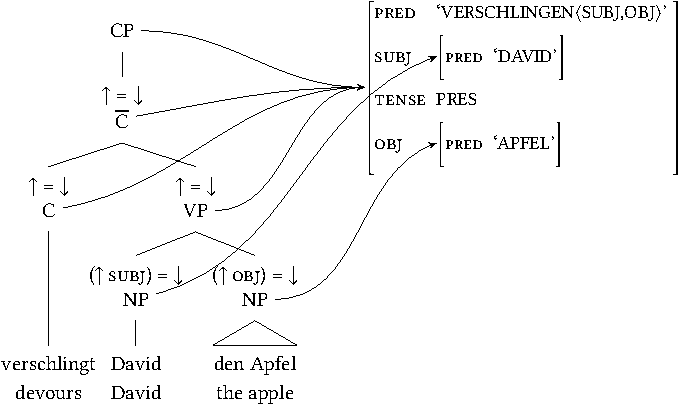
\includegraphics[width=.75\textwidth]{Figures/verschlingt-david-den-apfel-lfg-lsp-crop}}

\bigskip

\centerline{Analysis adapted from \citet[\page 41]{Berman2003a}.}

\vfill

}


\subsection{Local reordering}

\frame{
\frametitle{Local reordering}

\begin{itemize}
\item Two options are discussed:
\begin{itemize}
\item movement of arguments from a base configuration as in GB (see \citealp{Choi99a-u})
\pause
\item direct licensing by phrase structure rules (see Berman \citeyear[Section~2.1.3.1]{Berman96a-u}; \citeyear{Berman2003a})
\end{itemize}
\end{itemize}

}


\frame{
\frametitle{Local reordering as ``base generateion'' (I)}

\begin{itemize}
\item Case requirements are specified in lexical items:
\ea
\label{le-verschlingen}
\catlexentry{verschlingt}{V}{(\up\ \lfgpred) = {\small `VERSCHLINGEN\sliste{\lfgsubj, \lfgobj}'}\\*
                             (\up\ \lfgsubj{} {\small AGR CAS}) = NOM\\*
                             (\up\ \lfgobj{} {\small AGR CAS}) = ACC\\*
                             (\up\ \lfgtense) = \small PRES}
\z

\pause
\item GPSG: all arguments are combined with the head in one go.
\pause
\item LFG: no argument is combined with the verb and we get a VP without anything.

\ea
\label{LFG-v-vp}
\phraserule{VP}{
\rulenode{(V)\\* \up~=~\down}}
\z
\pause
\item Hm.
\pause
\item But this is just to get the recursion going.
\end{itemize} 


}


\frame{
\frametitle{Local reordering as ``base generateion'' (II)}

\begin{itemize}
\item Case requirements are specified in lexical items:
\ea
\label{le-verschlingen}
\catlexentry{verschlingt}{V}{(\up\ \lfgpred) = {\small `VERSCHLINGEN\sliste{\lfgsubj, \lfgobj}'}\\*
                             (\up\ \lfgsubj{} {\small AGR CAS}) = NOM\\*
                             (\up\ \lfgobj{} {\small AGR CAS}) = ACC\\*
                             (\up\ \lfgtense) = \small PRES}
\z

\ea
\label{LFG-v-vp}
\phraserule{VP}{
\rulenode{(V)\\* \up~=~\down}}
\z
\pause
\item Recursive rule to add NP arguments:
\ea
\label{lfg-vp-regel}
\phraserule{VP}{
\rulenode{NP\\* (\upsp \lfgsubj|\lfgobj|\objtheta) = \down}
\rulenode{VP\\* \up~=~\down}}
\z
\pause
\item similar rules for PP arguments and so on.

\end{itemize} 


}

\frame{
\frametitle{Binary branching with normal order (nom, acc)}


\bigskip

\centerline{%
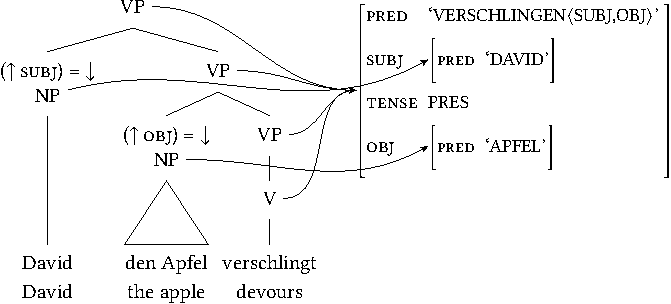
\includegraphics{Figures/david-den-apfel-verschlingt-lfg-lsp-crop}
}

\bigskip

%\centerline{Analysis adapted from \citet[\page 41]{Berman2003a}.}

\vfill

}

\frame{
\frametitle{Binary branching with marked order (acc, nom)}


\bigskip

\centerline{%
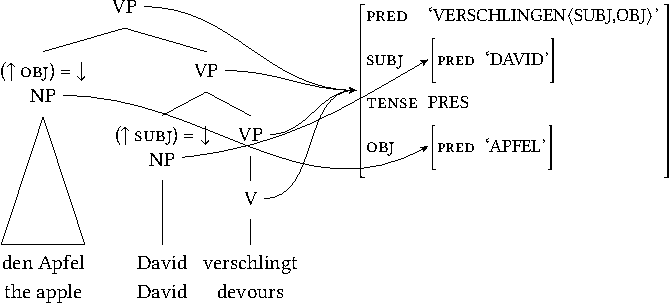
\includegraphics{Figures/den-apfel-david-verschlingt-lfg-lsp-crop}
}

\bigskip

%\centerline{Analysis adapted from \citet[\page 41]{Berman2003a}.}

\vfill

}




\subsection{Long"=distance dependencies}

\subsubsection{Discourse functions}


\frame{
\frametitle{Long"=distance dependencies: Discourse functions (I)}


\begin{itemize}
\item Observation: the displaced constituent \emph{Chris} is characterized by two functions:
\ea
Chris, we think that David saw.
\z

\begin{itemize}
\item an \alert{argument function} which is normally realized in a different position: the \lfgobj
  function of \emph{saw} 
\pause
\item a certain emphasis of the information"=structural status in this construction: \textsc{topic}
  in the matrix clause -- a \alert{discourse function}
\end{itemize}
\end{itemize}

}

\frame{
\frametitle{Discourse functions (II)}

\begin{itemize}
\item grammaticalized discourse functions: \textsc{topic} and \textsc{focus}\\
      (\textsc{subj} is a default discourse function).
  \begin{itemize}
  \item  Only 
\alert{grammaticalized} discourse functions are represented on the level of f"=structure, that is, those
that are created by a fixed syntactic mechanism and that interact with the rest of the syntax.

%%   (F\"ur die umfassende Repr\"asentation von informationsstrukturellen
%%   Eigenschaften wird in LFG eine separate Informationsstruktur
%%   angenommen.)
\pause
  \item Unlike argument functions, the discourse functions  \textsc{topic} and
\textsc{focus} are not lexically subcategorized and are therefore not
subject to the completeness and coherence conditions.
\pause
  \item \textsc{topic} and \textsc{focus} are identified with an
f"=structure that bears an argument function.
  \end{itemize}
\end{itemize}

}

\frame{
\frametitle{Discourse functions in f-structure}
\smallframe

\eal
\ex Chris, we think that David saw.
\ex 
\lfgms{ pred & `think\sliste{ \lfgsubj, \comp }' \\
        topic & \rnode{topic}{\lfgms{ pred & `Chris' \\
                                   }}\\[4mm]
        subj & \lfgms{ pred & `pro'\\
                     }\\
        comp & \lfgms{ pred & `see\sliste{ \lfgsubj, \lfgobj }\\
                       subj & \lfgms{ pred & `David' \\
                                    }\\
                       obj  & \rnode{obj}{}\\
                     }\\
      }
\nccurve[ncurv=2.2]{topic}{obj}
\zl

\bigskip
Der Strich sagt: The value of \textsc{topic} is identical to \textsc{comp obj}.

The constraint: (\up  \textsc{topic})=(\up \textsc{comp obj})
}

\frame{
\frametitle{Different levels of embedding (I)}

\eal
\ex Chris, we saw.
\ex 
\lfgms{ pred & `see\sliste{ \lfgsubj, \lfgobj }' \\
        topic & \rnode{topic}{\lfgms{ pred & `Chris' \\
                                   }}\\[4mm]
        subj & \lfgms{ pred & `pro'\\
                     }\\
        obj  & \rnode{obj}{}\\
      }
%\nodecurve[r]{topic}[r]{obj}{15em}
\nccurve[nodesepA=1pt,ncurv=2.2]{topic}{obj}
\zl

\bigskip

The constraint: (\up  \textsc{topic})=(\up \textsc{obj})
}


\frame{
\frametitle{Different levels of embedding (II)}
\smallframe

\eal
\ex Chris, we think Anna claims that David saw.
\ex 
\scalebox{0.85}{%
\lfgms{ pred & `think\sliste{ \lfgsubj, \comp }' \\
        topic & \rnode{topic}{\lfgms{ pred & `Chris' \\
                                   }}\\[4mm]
        subj & \lfgms{ pred & `pro'\\
                     }\\
        comp & \lfgms{ pred & `claim\sliste{ \lfgsubj, \comp }\\
                       subj & \lfgms{ pred & `Anna' \\
                                   }\\
                       comp & \lfgms{ pred & `see\sliste{ \lfgsubj, \lfgobj }\\
                                      subj & \lfgms{ pred & `David' \\
                                                   }\\
                                      obj  & \rnode{obj}{}\\
                                    }\\
                     }\\
      }
%\nodecurve[r]{topic}[r]{obj}{15em}%
\nccurve[ncurv=2.2]{topic}{obj}
}
\zl

The constraint: (\up  \textsc{topic})=(\up \textsc{comp comp obj})
}

\subsubsection{Functional uncertainty}

\frame{
\frametitle{Functional uncertainty}

\begin{itemize}
\item The constraints are c-structure constraints:

\ea
\begin{tabular}[t]{@{}ccc@{~=~}lc@{}}
CP & $\rightarrow$ & \multicolumn{2}{l}{\hspaceThis{(\up \textsc{topic})}XP} & C$'$ \\
 & &  (\up \textsc{topic}) & \down & \up=\down \\
 & &  (\up \textsc{topic}) & (\up \textsc{comp obj})\\
\end{tabular}
\z

\pause
\item But we have different levels of embedding:

\ea
(\up  \textsc{topic})=(\up \textsc{obj})\\
(\up  \textsc{topic})=(\up \textsc{comp obj})\\
(\up  \textsc{topic})=(\up \textsc{comp comp obj})\\
\ldots
\z

\pause
\item The generalization over these equations is:
\ea
(\up  \textsc{topic})=(\up \textsc{comp* obj})
\medskip
\z
The Kleene star `*' stands for arbitrarily many repetitions of \comp.

\end{itemize}

}

\frame{
\frametitle{Disjunctions and variables for grammatical functions}


\begin{itemize}[<+->]
\item The fronted element is not necessarily a \textsc{topic},
      \focus is possible as well.
\item It is possible to state disjunctions:
\ea
(\up  \textsc{topic$|$focus})=(\up \textsc{comp* obj})
\z
\item \textsc{topic$|$focus} can be abbreviated by using the shortcut \textsc{df} (discourse function).


%% \begin{tabular}{@{}ccc@{~=~}lc@{}}
%% CP & $\rightarrow$ & \multicolumn{2}{l}{\hspaceThis{(\up \textsc{topic})}XP} & C$'$ \\
%%  & &  (\up \textsc{DF}) & \down & \up=\down \\
%%  & &  (\up \textsc{DF}) & (\up \textsc{comp* GF})\\
%% \end{tabular}

\end{itemize}

}

\subsection{Summary}

\frame{
\frametitle{Summary}

\begin{itemize}
\item LFG is unification-based/constraint-based and works with feature structures and PSG rules.
\item Grammatical functions are primitives of LFG,\\
      they are not defined with reference to structure (as in GB)
\item LFG is strongly lexicalized. Valence alternations like passivization are captured in the
  lexicon via lexical rules.
\end{itemize}

}



%      <!-- Local IspellDict: en_US-w_accents -->
